\documentclass[aspectratio=169,11pt]{beamer}

% ---------- Packages ----------
\usepackage[T1]{fontenc}
\usepackage[utf8]{inputenc}
\usepackage{lmodern}
\usepackage{amsmath,amssymb}
\usepackage{booktabs}
\usepackage{array}
\usepackage{xcolor}
\usepackage{graphicx}
\usepackage{hyperref}
\usepackage{tikz}
\usetikzlibrary{arrows.meta,positioning,shapes.geometric}

% ---------- Minimal Theme ----------
\usetheme{default}
\usecolortheme{default}
\setbeamertemplate{navigation symbols}{}
\setbeamertemplate{itemize items}[square]
\setbeamertemplate{enumerate items}[default]

% Reduce margins
\setbeamersize{text margin left=0.5cm, text margin right=0.5cm}

% Color palette: professional and minimal
\definecolor{darkgray}{RGB}{45,45,45}
\definecolor{accent}{RGB}{15,75,145}
\definecolor{lightgray}{RGB}{240,240,240}
% Keep old colors mapped to minimal palette for backward compatibility
\definecolor{softorange}{RGB}{245,235,220}
\definecolor{softblue}{RGB}{230,240,250}
\definecolor{softgreen}{RGB}{230,245,240}

% Minimal frame styling
\setbeamercolor{structure}{fg=darkgray}
\setbeamercolor{frametitle}{fg=darkgray,bg=}
\setbeamercolor{title}{fg=darkgray,bg=}
\setbeamercolor{subtitle}{fg=darkgray}
\setbeamercolor{block title}{fg=white,bg=accent}
\setbeamercolor{block body}{bg=lightgray!15,fg=darkgray}

% Reduce spacing around blocks
\addtobeamertemplate{block begin}{\vskip-0.5em}{}
\addtobeamertemplate{block end}{\vskip-0.3em}{}

% Alert block styling
\setbeamercolor{alerted text}{fg=darkgray}
\setbeamercolor{alertblock title}{fg=white,bg=darkgray}
\setbeamercolor{alertblock body}{bg=lightgray!10,fg=darkgray}
\addtobeamertemplate{alertblock begin}{\vskip-0.5em}{}
\addtobeamertemplate{alertblock end}{\vskip-0.3em}{}
\setbeamercolor{background canvas}{bg=white}

\setbeamerfont{frametitle}{size=\large,series=\bfseries}
\setbeamerfont{title}{size=\Large,series=\bfseries}
\setbeamerfont{subtitle}{size=\normalsize}
\setbeamerfont{block title}{size=\normalsize,series=\bfseries}

% Minimal frame header with tight spacing
\setbeamertemplate{frametitle}{
  \vskip0.5em
  \insertframetitle
  \vskip-0.6em
  {\color{accent}\rule{\textwidth}{1.5pt}}
  \vskip-0.1em
}

% Add slide numbers in bottom right
\setbeamertemplate{footline}{
  \hfill\insertframenumber\hspace{0.5em}\vspace{0.3em}
}

\newcommand{\tagbox}[2]{%
  \begin{tikzpicture}[baseline=(X.base)]
    \node[rounded corners=2pt, fill=#1, inner xsep=5pt, inner ysep=2pt] (X) {\small\bfseries #2};
  \end{tikzpicture}%
}

\newcommand{\tightitems}{\setlength{\itemsep}{0.25em}\setlength{\parskip}{0pt}}
\newlength{\grpoformulawidth}

% ---------- Metadata ----------
\title{Reinforcement Learning for Long-Context Reasoning}
\subtitle{Hierarchical Agent Architecture with Decomposed Rewards}
\author{Arjun Vaidya \and Peter Driscoll}
\date{May 2026}

\begin{document}

% ---------- Slide 1 ----------
\begin{frame}
  \titlepage
\end{frame}

% ---------- Slide 2: Introduction ----------
\begin{frame}{The Problem}
\begin{block}{Mathematical Reasoning Challenge}
Large language models struggle with multi-step reasoning [1]. \newline
Chain-of-thought helps, but better training methods are needed.
\end{block}

\vspace{0.8em}
\begin{columns}[T,onlytextwidth]
  \begin{column}{0.48\textwidth}
    \begin{block}{Our Solution}
      Use RL to incentivize the model towards the right distribution of reasoning and solving behaviors, without a separate value network.

      \vspace{0.6em}
      \textbf{Methods:} \\ Hierarchical decomposition, GRPO [2], decomposed rewards
      \vfill
    \end{block}
  \end{column}
  \begin{column}{0.48\textwidth}
    \begin{block}{The Bigger Challenge}
      Prior work (CoT [1], GRPO [2], hierarchical agents [3]) show promise.

      \vspace{1.5em}
      \textbf{Challenge:} \\ Decoupling rewards between reasoning and solving phases while maintaining signal flow.
    \end{block}
  \end{column}
\end{columns}
\end{frame}

% ---------- Slide 3: Dataset ----------
\begin{frame}{Dataset: GSM8K}
\begin{columns}[T,onlytextwidth]
  \begin{column}{0.48\textwidth}
    \begin{block}{Overview}
      \begin{itemize}\tightitems
        \item 8.5K grade-school math word problems.
        \item Linguistically diverse prompts requiring multi-step reasoning.
        \item Answers include chain-of-thought style reasoning plus a final numeric target.
      \end{itemize}
    \end{block}
  \end{column}
  \begin{column}{0.48\textwidth}
    \begin{block}{Data Structure}
      \begin{itemize}\tightitems
        \item \textbf{Question:} math word problem.
        \item \textbf{Answer / reasoning:} step-by-step solution logic.
        \item \textbf{Final answer:} numeric label, often marked with \texttt{\#\#\#\#}.
      \end{itemize}
    \end{block}
  \end{column}
\end{columns}

\vspace{0.8em}
\begin{block}{How We Use It}
\begin{itemize}\tightitems
  \item Fine-tune on the \texttt{train} split.
  \item Extract exact numeric answers for automated grading and reward computation.
\end{itemize}
\end{block}
\end{frame}

% ---------- Slide 3 ----------
\begin{frame}{Baseline: Reward-Weighted Supervised Fine-Tuning}
\begin{columns}[T,onlytextwidth]
  \begin{column}{0.52\textwidth}
    \begin{block}{Flat Baseline}
    \begin{itemize}\tightitems
      \item Standard causal language model.
      \item No routing or expert-selection mechanism.
      \item Custom \texttt{RewardWeightedTrainer} for supervised fine-tuning.
    \end{itemize}
    \end{block}

    \begin{block}{Efficiency Choice}
    \begin{itemize}\tightitems
      \item LoRA adapters target attention projections.
      \item Main targets: \texttt{q\_proj} and \texttt{v\_proj}.
    \end{itemize}
    \end{block}
  \end{column}
  \begin{column}{0.44\textwidth}
    \begin{block}{Training Objective}
      \begin{enumerate}\tightitems
        \item Format examples as: \texttt{Question: [Q] \textbackslash n Reasoning: [A]}.
        \item Assign binary reward from numeric-answer format.
        \item Weight sequence cross-entropy by reward.
      \end{enumerate}
    \end{block}

    \vspace{0.4em}
    \centering
    \tagbox{softorange}{$\mathcal{L}=R(x,y)\,\mathcal{L}_{\mathrm{CE}}(x,y)$}
  \end{column}
\end{columns}
\end{frame}

% ---------- Slide 4 ----------
\begin{frame}{Why Direct RL Over SFT?}
\begin{columns}[T,onlytextwidth]
  \begin{column}{0.47\textwidth}
    \begin{block}{Computational Efficiency}
    \begin{itemize}\tightitems
      \item Skip an intermediate SFT stage.
      \item Optimize directly against task reward.
      \item Reduce mismatch between training objective and evaluation objective.
    \end{itemize}
    \end{block}
  \end{column}
  \begin{column}{0.47\textwidth}
    \begin{block}{Alignment Benefits}
    \begin{itemize}\tightitems
      \item Avoid overfitting to human-curated SFT traces.
      \item Learn from the reward signal that actually defines success.
      \item Useful when correct outputs can be automatically checked.
    \end{itemize}
    \end{block}
  \end{column}
\end{columns}

\vfill
\begin{center}
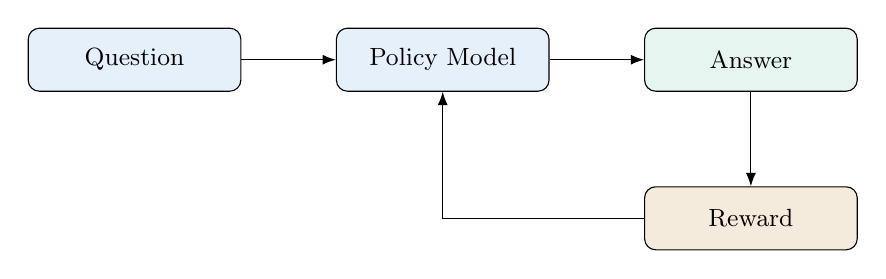
\begin{tikzpicture}[node distance=1.2cm, every node/.style={font=\small}]
  \node[draw,rounded corners,fill=softblue,minimum width=2.7cm,minimum height=0.8cm] (q) {Question};
  \node[draw,rounded corners,fill=softblue,right=of q,minimum width=2.7cm,minimum height=0.8cm] (model) {Policy Model};
  \node[draw,rounded corners,fill=softgreen,right=of model,minimum width=2.7cm,minimum height=0.8cm] (ans) {Answer};
  \node[draw,rounded corners,fill=softorange,below=of ans,minimum width=2.7cm,minimum height=0.8cm] (rew) {Reward};
  \draw[-{Latex}] (q) -- (model);
  \draw[-{Latex}] (model) -- (ans);
  \draw[-{Latex}] (ans) -- (rew);
  \draw[-{Latex}] (rew.west) -| (model.south);
\end{tikzpicture}
\end{center}
\vfill
\end{frame}

% ---------- Slide 5 ----------
\begin{frame}{GRPO: Eliminating the Critic Network}
\begin{columns}[T,onlytextwidth]
  \begin{column}{0.40\textwidth}
    \begin{block}{Traditional PPO}
    \begin{itemize}\tightitems
      \item Requires a separate critic network.
      \item Critic estimates per-step value functions.
      \item Adds memory, compute, and tuning overhead.
    \end{itemize}
    \end{block}
  \end{column}
  \begin{column}{0.58\textwidth}
    \begin{block}{GRPO Idea}
    \begin{itemize}\tightitems
      \item Sample a group of responses for the same prompt.
      \item Compare within-group and normalize rewards.
    \end{itemize}
    \end{block}

    \vspace{0.6em}
    \settowidth{\grpoformulawidth}{\tagbox{softgreen}{$A_i=\dfrac{R(r_i)-\mathrm{mean}(R)}{\mathrm{std}(R)}$}}
    \begin{center}
    \small\tagbox{softgreen}{$A_i=\dfrac{R(r_i)-\mathrm{mean}(R)}{\mathrm{std}(R)}$}
    \end{center}
    \vspace{0.6em}
    \noindent\hspace*{\dimexpr0.5\linewidth-0.5\grpoformulawidth\relax}
    \begin{minipage}[t]{\grpoformulawidth}
    \raggedright
    \small
    \tagbox{softblue}{No value model}\\[1.3em]
    \tagbox{softgreen}{Lower overhead}\\[1.3em]
    \tagbox{softorange}{Sequence-level credit}
    \end{minipage}

    
  \end{column}
\end{columns}
\end{frame}

% ---------- Slide 6 ----------
\begin{frame}{Router Reward: Outcome-Only vs. Process-Based}
\begin{columns}[T,onlytextwidth]
  \begin{column}{0.48\textwidth}
    \begin{block}{Outcome-Only Reward}
    \begin{itemize}\tightitems
      \item $R=1$ if final answer matches ground truth.
      \item $R=0$ if final answer is incorrect.
      \item Easy to implement and cheap to compute.
      \item Weakness: gives no feedback on intermediate planning quality.
    \end{itemize}
    \end{block}
  \end{column}
  \begin{column}{0.48\textwidth}
    \begin{block}{Process Reward Models}
    \begin{itemize}\tightitems
      \item Score each planning step independently.
      \item Evaluate clarity, concreteness, and logical order.
      \item Can detect poor plans before final execution fails.
      \item Weakness: requires step-level quality metrics.
    \end{itemize}
    \end{block}
  \end{column}
\end{columns}

\vspace{0.8em}
\begin{alertblock}{Core Tradeoff}
Outcome rewards are simple but sparse. Process rewards are richer but harder to define without adding noise or reward hacking.
\end{alertblock}
\end{frame}

% ---------- Slide 7 ----------
\begin{frame}{Conditional and Hybrid Router Rewards}
\begin{block}{Conditional Reward Modeling}
\begin{itemize}\tightitems
  \item Scores a step based on preceding steps and the final outcome.
  \item Asks whether the plan would work if executed perfectly.
  \item Checks for necessary quantities, correct decomposition, and logical order.
  \item Captures inter-step dependencies but makes credit assignment more complex.
\end{itemize}
\end{block}

\vspace{0.6em}
\begin{block}{Practical Hybrid Reward}
\begin{center}
\Large
\tagbox{softorange}{$R_{\mathrm{hybrid}}=0.5\,R_{\mathrm{plan}}+0.5\,R_{\mathrm{outcome}}$}
\end{center}
\begin{itemize}\tightitems
  \item Balances structure and correctness.
  \item Gives smoother learning signal than outcome-only reward.
  \item Lowest-cost starting point for router reward development.
\end{itemize}
\end{block}
\end{frame}

% ---------- Slide 8 ----------
\begin{frame}{LLM-as-Judge: Expert Plan Evaluation}
\begin{columns}[T,onlytextwidth]
  \begin{column}{0.48\textwidth}
    \begin{block}{How It Works}
    \begin{enumerate}\tightitems
      \item Router generates a structured plan.
      \item Send question and plan to Claude with an evaluation prompt.
      \item Score clarity, completeness, and feasibility from 0 to 10.
      \item Convert to $[0,1]$ and blend with outcome reward.
    \end{enumerate}
    \end{block}
  \end{column}
  \begin{column}{0.48\textwidth}
    \begin{block}{Strengths and Limits}
    \begin{itemize}\tightitems
      \item \textbf{Strength:} catches subtle plan errors missed by heuristics.
      \item \textbf{Strength:} no reward model training required.
      \item \textbf{Limit:} slower because it requires API calls.
      \item \textbf{Limit:} cost and non-determinism make it risky for high-volume training.
    \end{itemize}
    \end{block}
  \end{column}
\end{columns}
\vspace{0.7em}
\begin{block}{Practical Strategy}
Train with fast heuristic rewards and validate with an LLM judge to detect reward inflation, reward deflation, and brittle heuristic behavior.
\end{block}
\end{frame}

% ---------- Slide 9 ----------
\begin{frame}{W\&B Training Results}
\begin{block}{Logged source}
\small
W\&B run: \texttt{run-20260505\_080608-j7h3rnpx} (slim pass, \texttt{B=120}, \texttt{G=2}, 35 steps).
\end{block}

\vspace{0.4em}
\begin{center}
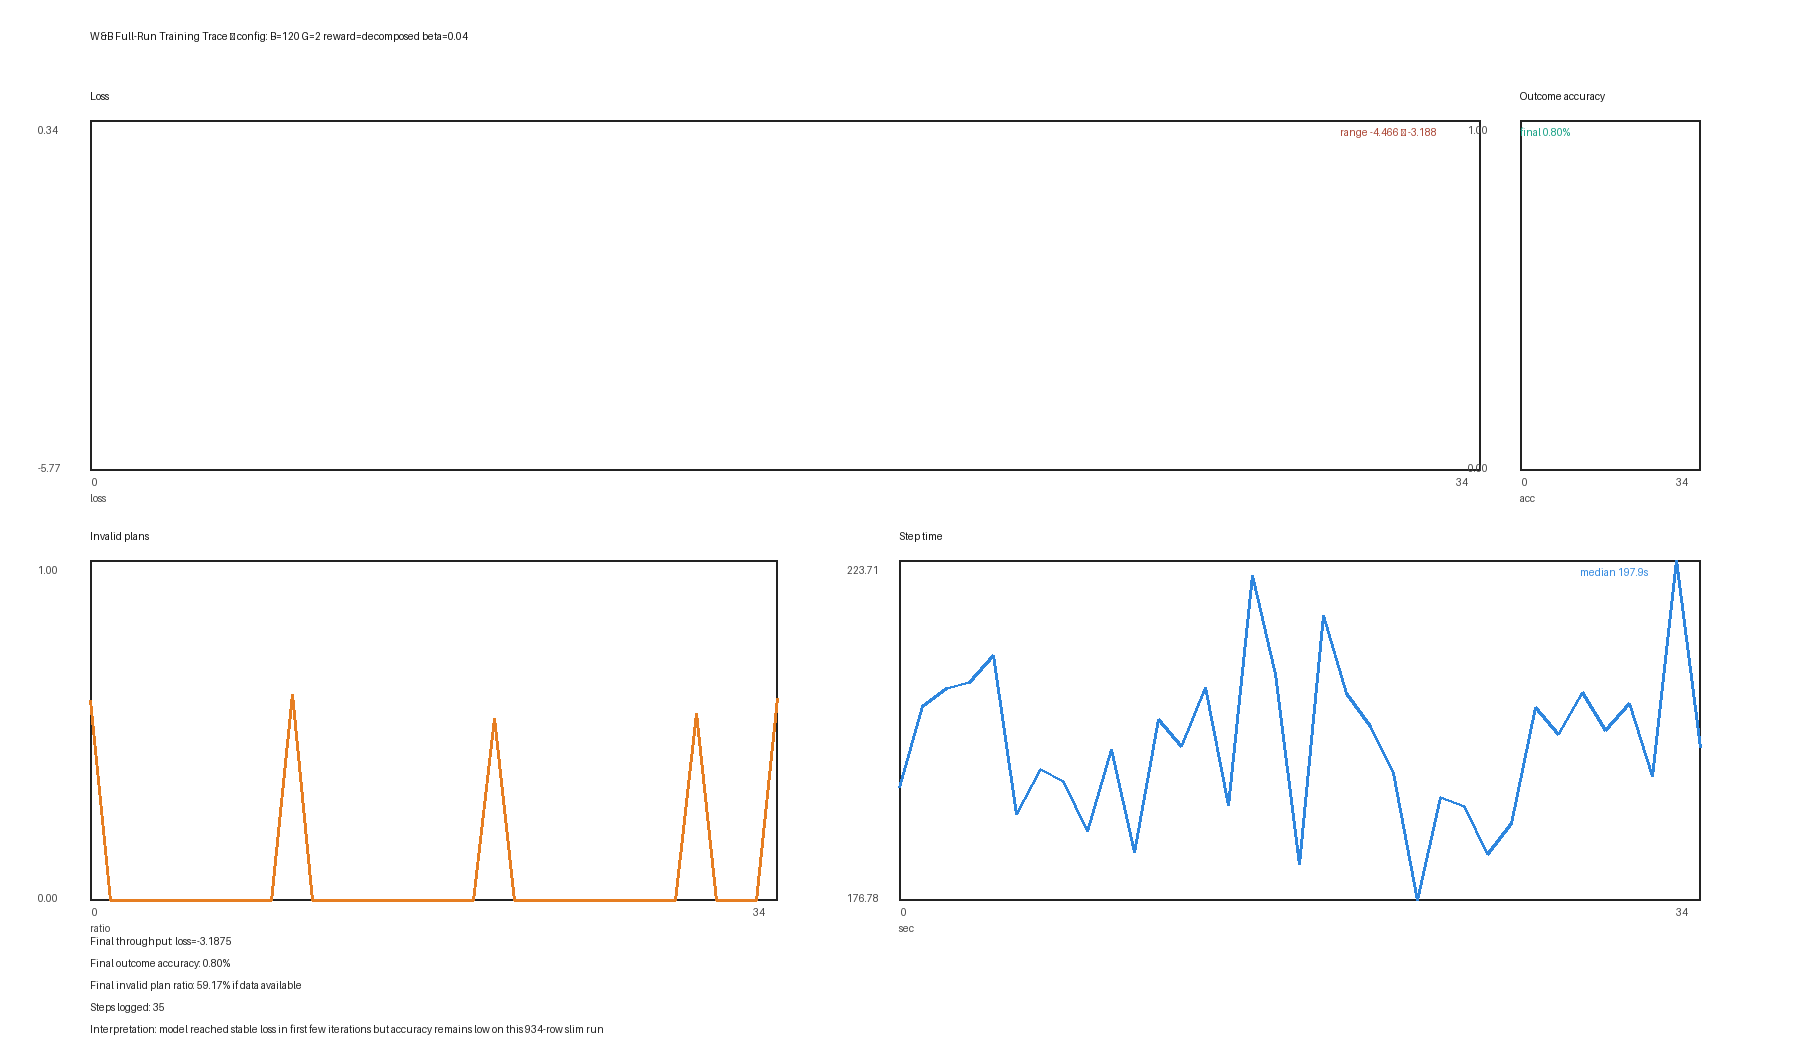
\includegraphics[width=\textwidth]{../../docs/assets/wandb_training_results_chart.png}
\end{center}

\vspace{0.2em}
\begin{columns}[T,onlytextwidth]
  \begin{column}{0.58\textwidth}
    \begin{itemize}\tightitems
      \item Loss moved rapidly in the first 10 steps but stays high-variance, consistent with sparse reward feedback.
      \item Outcome accuracy remains low and flat (roughly 0.8\%--1.7\% on this run), indicating little signal-to-signal generalization yet.
      \item Invalid plans hover in the same band as rollout volume rises, confirming a quality-control bottleneck before reward optimization.
    \end{itemize}
  \end{column}
  \begin{column}{0.40\textwidth}
    \begin{alertblock}{Operational takeaway}
      Use this as the throughput/perf baseline:
      keep the same rollout infrastructure, and focus next on reward shaping and planner quality before scaling steps.
    \end{alertblock}
  \end{column}
\end{columns}
\end{frame}

% ---------- Slide 10 ----------
\begin{frame}{References}
\small
\begin{itemize}\tightitems
  \item [1] Wei, J., Wang, X., et al. \textit{Chain-of-Thought Prompting Elicits Reasoning in Large Language Models}. NeurIPS 2023. \url{https://arxiv.org/abs/2201.11903}

  \item [2] DeepSeek Team. \textit{DeepSeek-R1: Incentivizing Reasoning Capability in LLMs via Reinforcement Learning}. 2025. \url{https://arxiv.org/pdf/2501.12948}

  \item [3] Weng, L. \textit{LLM Powered Autonomous Agents}. Blog Post, 2023. \url{https://lilianweng.github.io/posts/2023-06-23-agent/}

  \item [4] Zhang et al. \textit{ReST-MCTS*: LLM Self-Training via Process Reward Guided Tree Search}. NeurIPS 2024. \url{https://arxiv.org/abs/2406.03816}

  \item [5] \textit{Linking Process to Outcome: Conditional Reward Modeling for LLM Reasoning}. \url{https://arxiv.org/abs/2509.26578}
\end{itemize}
\end{frame}

\end{document}
